\documentclass[10pt, compress, aspectratio=169]{beamer}

\usetheme[numbering=fraction, progressbar=none, titleformat=smallcaps]{metropolis}
\usepackage{booktabs}
\usepackage{array}
\usepackage{listings}
\usepackage{graphicx}
\usepackage[scale=2]{ccicons}
\usepackage{url}
\usepackage{relsize}
\usepackage{wasysym}

\usepackage{pgfplots}
\usepgfplotslibrary{dateplot}

\lstset{ %
  backgroundcolor={},
  basicstyle=\ttfamily\footnotesize,
  breakatwhitespace=true,
  breaklines=true,
  captionpos=n,
  commentstyle=\color{orange},
  escapeinside={\%*}{*)},
  extendedchars=true,
  frame=n,
  keywordstyle=\color{orange},
  language=C++,
  rulecolor=\color{black},
  showspaces=false,
  showstringspaces=false,
  showtabs=false,
  stepnumber=2,
  stringstyle=\color{gray},
  tabsize=2,
  keywords={thrust,plus,device_vector, copy,transform,begin,end, copyin,
  copyout, acc, \_\_global\_\_, void, int, float, main, threadIdx, blockIdx,
  blockDim, if, else, malloc, NULL, cudaMalloc, cudaMemcpy, cudaSuccess,
  cudaGetLastError, cudaDeviceSynchronize, cudaFree, cudaMemcpyDeviceToHost,
  cudaMemcpyHostToDevice, const, data, independent, kernels, loop,
  fprintf, stderr, cudaGetErrorString, EXIT_FAILURE, for, dim3},
  otherkeywords={::, \#pragma, \#include, <<<,>>>, \&, \*, +, -, /, [, ], >, <}
}

\renewcommand*{\UrlFont}{\ttfamily\smaller\relax}

\graphicspath{{images/}}

\title{Builtin commands}
\author{\footnotesize Rodrigo Siqueira \\ {\scriptsize siqueira@ime.usp.br}}
\institute{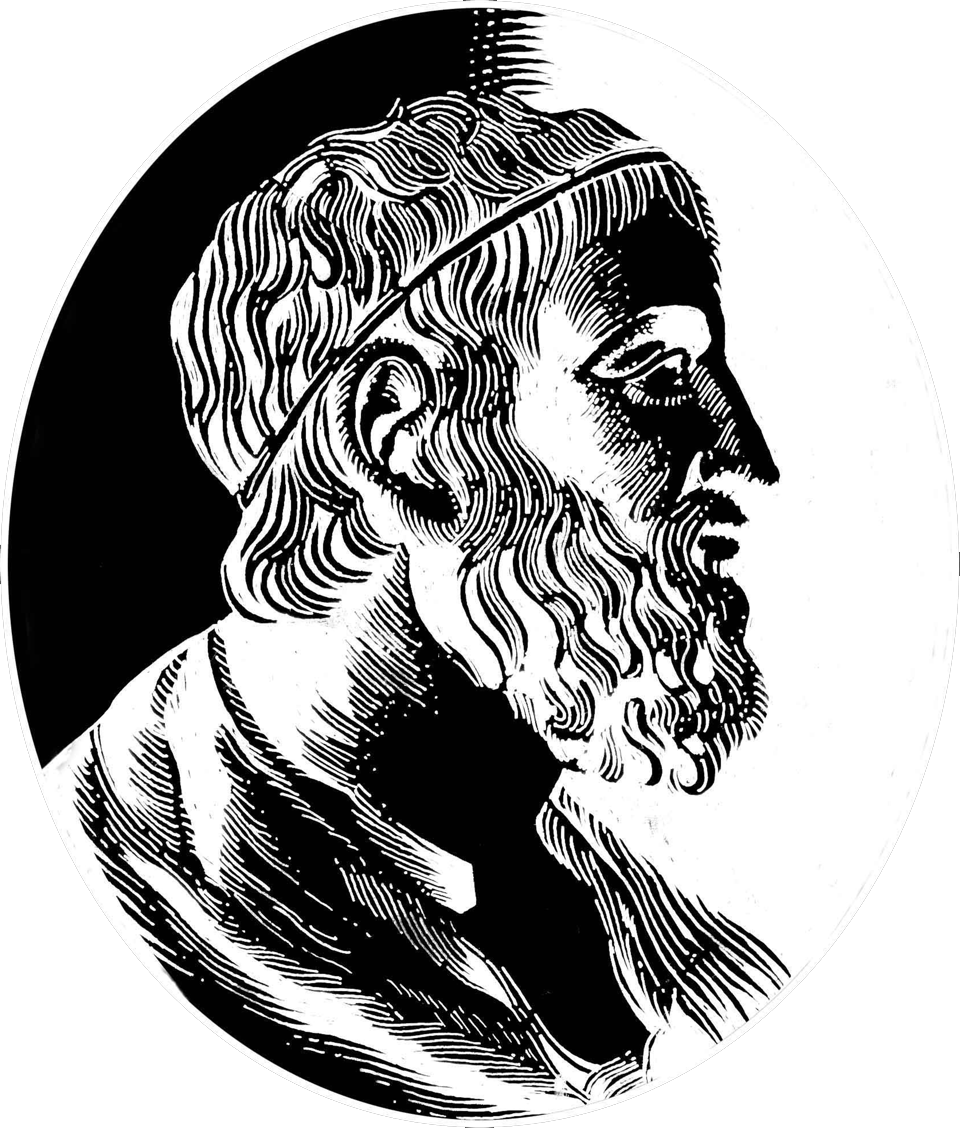
\includegraphics[height=2cm]{imelogo}\\[0.2cm] Department of Computer Science \\ University of São Paulo}

\begin{document}

\maketitle

%------------------------------------------------------------------------------
\section{Introduction}
\begin{frame}{Overview}
  % TODO: Create this section
  \begin{itemize}
    \item Computers...
  \end{itemize}
\end{frame}

%------------------------------------------------------------------------------
\section{Bourne Shell Builtin}
\begin{frame}{Colon (:)}
\end{frame}

\begin{frame}{Dot (.)}
\end{frame}

\begin{frame}{break}
  \metroset{block=fill}
  \begin{alertblock}{Syntax}
    break [n]
  \end{alertblock}

  \lstinputlisting{codes/break_with_n.sh}
\end{frame}

\begin{frame}{cd}
  \metroset{block=fill}
  \begin{alertblock}{Syntax}
    cd [-L|[-P[-e]] [-@] [dir]
  \end{alertblock}
\end{frame}

\begin{frame}{continue}
  \metroset{block=fill}
  \begin{alertblock}{Syntax}
    continue [n]
  \end{alertblock}
  \lstinputlisting{codes/continue_with_n.sh}
\end{frame}

\begin{frame}{eval}
  \metroset{block=fill}
  \begin{alertblock}{Syntax}
    eval [arguments]
  \end{alertblock}
  \lstinputlisting{codes/eval_example.sh}
\end{frame}

\begin{frame}{exec}
  \metroset{block=fill}
  \begin{alertblock}{Syntax}
    exec [-cl] [-a name] [command] [arg]
  \end{alertblock}
  \lstinputlisting{codes/exec_input.sh}
\end{frame}

\begin{frame}{exit}
  \metroset{block=fill}
  \begin{alertblock}{Syntax}
    exit [n]
  \end{alertblock}
\end{frame}

\begin{frame}{export}
  \metroset{block=fill}
  \begin{alertblock}{Syntax}
    export [-fn] [-p] [name[=value]]
  \end{alertblock}
\end{frame}

\begin{frame}{getopts}
  \metroset{block=fill}
  \begin{alertblock}{Syntax}
    getopts "options" name [arg]
  \end{alertblock}
  \lstinputlisting{codes/getopts_simple.sh}
\end{frame}

\begin{frame}{hash}
  \metroset{block=fill}
  \begin{alertblock}{Syntax}
    hash [-r] [-p file] [-dt] [name]
  \end{alertblock}
\end{frame}

\begin{frame}{pwd}
  \metroset{block=fill}
  \begin{alertblock}{Syntax}
    pwd [-LP]
  \end{alertblock}
\end{frame}

\begin{frame}{readonly}
  \metroset{block=fill}
  \begin{alertblock}{Syntax}
    readonly [-aAf] [-p] [name[=value]] ...
  \end{alertblock}
\end{frame}

\begin{frame}{return}
  \metroset{block=fill}
  \begin{alertblock}{Syntax}
    return [n]
  \end{alertblock}
\end{frame}

\begin{frame}{shift}
  \metroset{block=fill}
  \begin{alertblock}{Syntax}
    shift [n]
  \end{alertblock}
\end{frame}

\begin{frame}{test}
  \metroset{block=fill}
  \begin{alertblock}{Syntax}
    test expression
  \end{alertblock}
\end{frame}

\begin{frame}{time}
  \metroset{block=fill}
  \begin{alertblock}{Syntax}
    time
  \end{alertblock}
\end{frame}

\begin{frame}{trap}
  \metroset{block=fill}
  \begin{alertblock}{Syntax}
    trap [-lp] [arg] [sigspec...]
  \end{alertblock}
  \lstinputlisting{codes/trap_simple.sh}
\end{frame}

%------------------------------------------------------------------------------
\section{Bash builtin}
\begin{frame}{alias}
  \metroset{block=fill}
  \begin{alertblock}{Syntax}
    alias [-p] [name[=value]...]
  \end{alertblock}
\end{frame}

\begin{frame}{bind}
  \metroset{block=fill}
  \begin{alertblock}{Syntax}
    bind [-m keymap] [-lpsvPSVX]
  \end{alertblock}
\end{frame}

\begin{frame}{builtin}
  \metroset{block=fill}
  \begin{alertblock}{Syntax}
    builtin [shell-builtin [args]]
  \end{alertblock}
\end{frame}

\begin{frame}{caller}
  \metroset{block=fill}
  \begin{alertblock}{Syntax}
    caller [expression]
  \end{alertblock}
  \lstinputlisting{codes/caller_test.sh}
\end{frame}

\begin{frame}{command}
  \metroset{block=fill}
  \begin{alertblock}{Syntax}
    command [-pVv] command [arguments ...]
  \end{alertblock}
\end{frame}

\begin{frame}{declare}
  \metroset{block=fill}
  \begin{alertblock}{Syntax}
    declare [-aAfFgilnrtux] [-p] [name[=value]...]
  \end{alertblock}
\end{frame}

\begin{frame}{echo}
  \metroset{block=fill}
  \begin{alertblock}{Syntax}
    echo [-neE] [args...]
  \end{alertblock}
\end{frame}

\begin{frame}{enable}
  \metroset{block=fill}
  \begin{alertblock}{Syntax}
    enable [-a] [-dnps] [-f filename] [name...]
  \end{alertblock}
\end{frame}

\begin{frame}{help}
  \metroset{block=fill}
  \begin{alertblock}{Syntax}
    help [-dms] [pattern]
  \end{alertblock}
\end{frame}

\begin{frame}{let}
  \metroset{block=fill}
  \begin{alertblock}{Syntax}
    let expression [expression...]
  \end{alertblock}
\end{frame}

\begin{frame}{local}
  \metroset{block=fill}
  \begin{alertblock}{Syntax}
    local [option] name[=value]
  \end{alertblock}
\end{frame}

\begin{frame}{logout}
\end{frame}

\begin{frame}{mapfile}
\end{frame}

\begin{frame}{printf}
  \metroset{block=fill}
  \begin{alertblock}{Syntax}
    printf [-v var] format [args]
  \end{alertblock}
\end{frame}

\begin{frame}{read}

\end{frame}

\begin{frame}{readarray}
\end{frame}

\begin{frame}{source}
\end{frame}

\begin{frame}{type}
  \metroset{block=fill}
  \begin{alertblock}{Syntax}
    type [-afptP] [name]
  \end{alertblock}
\end{frame}

\begin{frame}{typeset}
\end{frame}

\begin{frame}{ulimit}
\end{frame}

%------------------------------------------------------------------------------
\section{About this presentation}
\begin{frame}[standout]
  % TODO: Improve it
   \begin{center}\ccbysa\end{center}
\end{frame}

%TODO: Bibliography
% break [n]: http://tldp.org/LDP/abs/html/loopcontrol.html
% continue [n]: http://tldp.org/LDP/abs/html/loopcontrol.html
% exec: http://wiki.bash-hackers.org/commands/builtin/exec
% caller: http://wiki.bash-hackers.org/commands/builtin/caller
\maketitle

\end{document}
